% Thesis paper
% submitting to RV 2015
% spring 2015
% Aaron Kane

%\documentclass[]{Z:/Private/research/TeX/llncs/llncs}
\documentclass[]{llncs}
%\documentclass[]{C:/Users/akane/Documents/Research/TeX/llncs/llncs}
%% loading some packages, deleted all the info text from the ieee example page
\usepackage[nocompress]{cite}
\usepackage[cmex10]{amsmath}
\usepackage{amssymb}
\usepackage{url}
\usepackage{multirow}
% restore ieee style page breaks over multiline equations
%\interdisplaylinepenalty=2500
\usepackage{array}
\usepackage[table]{xcolor}
\usepackage[font=footnotesize,caption=false]{subfig}	% subfigures
%\usepackage{fixltx2e} 		% fixes ordering of single/double column figures
%% a couple packages we might want, but don't want to load yet
%\usepackage{algorithmic}
%\usepackage{eqparbox}
%\usepackage{syntax-mdw}
\usepackage{listings}
\usepackage[pdftex]{graphicx}
\graphicspath{{../pdf/}{../jpeg/}}
\DeclareGraphicsExtensions{.pdf,.jpeg,.png}


%\addtolength{\textfloatsep}{-3.5cm}
%\addtolength{\floatsep}{-5cm}
\addtolength{\intextsep}{-5pt}
\addtolength{\belowcaptionskip}{-21pt}
%\usepackage{setspace}
%\doublespace
\usepackage{algorithmic}


% proof/theorem stuff
%\newtheorem{thm}{Theorem}
%\newtheorem{tdef}{Definition}
%\newtheorem{lemma}{Lemma}
%\newtheorem{case}{Case}

% defines
\newcommand{\rp}[2]{\ensuremath{\langle #1, #2 \rangle}}
\newcommand{\res}[2]{\ensuremath{r_{#1}^{#2}}}
\newcommand{\agmon}{\ensuremath{\mathbf{agmon}}}
\newcommand{\precis}{\textit{pr\`ecis}}
\newcommand{\pst}{\ensuremath{S^i_\psi}}
\newcommand{\rpt}[3]{\ensuremath{\langle #1, #2 \rangle}_{#3}}
\newcommand{\greduce}{\textit{reduce}}

%%%%%%%%%%%%%% end preamble, begin doc %%%%%%%%%%%%%%%%%%%%%%%%%%%%%%%%%
\begin{document}

% paper title
% can use linebreaks \\ within to get better formatting as desired
\title{Runtime Monitoring for Safety-Critical Embedded Systems}


\author{Aaron Kane \and Omar Chowdhury \and Philip Koopman}
\institute{Carnegie Mellon University, Pittsburgh, PA\\ \email{akane@cmu.edu, koopman@cmu.edu}}



% make the title area
\maketitle


\begin{abstract}
The trend towards increasing commercial-off-the-shelf (COTS) components in complex safety-critical systems is increasing the difficulty of verifying system correctness. 
Runtime verification (RV) is a lightweight technique to verify that certain properties hold over execution traces.
%
RV is usually implemented as runtime monitors that can be used as runtime fault detectors or test oracles to analyze a system under test for bad behaviors.
%
Most existing RV methods utilize some form of system or code instrumentation and thus are not designed to monitor potentially black-box COTS components.

%% major points to push
%
% dynamic programming algorithm
% 	also rewriting-based to a point
% embedded runtime monitor 
%	handles black-box systems
% 	reasonable overhead
%	aggressive monitoring, future/past (some specifications get checked faster in future then past)
% semi-formal mapping!!
%	remember, others do it, but noone is explicit
%
\end{abstract}


\section{Introduction}
Embedded systems, from home appliances to automobiles, are becoming increasingly complex due to the addition of new advanced features. 
Even traditionally non-critical systems are becoming safety- or mission-critical due to the addition of connectivity, complex autonomy and software reliant control (e.g., X-by-wire \cite{Leen2002}).
%
As more embedded systems become safety-critical, it is imperative that developers have methods to ensure that these systems are correct. 

Runtime verification (RV) is a more lightweight method aimed at verifying that a specific execution of a system satisfies or violates a given critical property \cite{Leucker2009}. 
%
Runtime verification can provide a formal analysis while avoiding many of the pitfalls that traditional model-based methods have such as state space explosion and model abstractions. 

The current trend in safety-critical embedded system is towards faster design cycles and more commercial-off-the-shelf (COTS) components. Being able to verify that a system made up of diverse components from multiple suppliers is safe and works correctly is difficult, even without the lack of design information that is inherent of COTS black-box components.
%
Runtime verification is a useful tool to help the verification of these systems. Runtime monitors can detect not only software faults but also hardware and design faults. 

Though there is an increasing focus on runtime monitors for safety-critical real-time systems, there is still little work aimed at monitoring systems with black-box components. This paper presents an end-to-end framework for monitoring safety-critical systems made of potentially black-box components. 
We present an external, broadcast bus monitor which primarily targets Controller Area Network (CAN), a common broadcast bus network used in modern automobiles and other ground vehicles. 

%
% 
%
%

\section{Background}
	% the robustness monitor approach in RV2014 is close to invariants
	% if you define your invariants well (and potentially add different levels of failures (e.g., warnings) you'd get to the same place
	% they require a predictive component in the system  -- we just want envelope
	% horizon is delay
	% observation map is semi-formal mapping

\subsubsection{Monitoring Safety-Critical Embedded Systems}
\label{sec:bg:sc_monitor}
Goodloe and Pike present a thorough survey of monitoring distributed real-time systems in \cite{Goodloe2010}. Notably, they present a set of monitor architecture constraints and propose three abstract monitor architectures in the context of monitoring these types of systems.
%
In \cite{Pike2011} Pike et. al update these constraints with the acronym ``FaCTS'': Functionality, Certifiability, Timing, and SWaP (size, weight and power). 
The Functionality constraint demands that a monitor cannot change the system under observation's (SUO's) behavior unless the target has violated the system specification. 
The Timing constraint similarly says that the monitor can not interfere with the non-faulty SUO's timing (e.g., task period/deadlines).
The Certifiability constraint is a softer constraint, arguing that a monitor should not make re-certification of SUO onerous. This is important because certification can be a major portion of design cost for these systems and nominally simple changes/additions to the SUO can require a broad and costly recertification.
Lastly, safety critical systems are often extremely cost sensitive with tight tolerances for additional physical size, weight or required power. Any monitor we wish to add to an existing system must fit within these existing tolerances.

%The three monitor architectures proposed by Goodloe and Pike are the Bus-Monitor Architecture, the single process monitor architecture, and the distributed process monitor architecture. 
One of Goodloe and Pike's proposed distributed real-time system monitor architectures is the bus-monitor architecture.
The bus monitor architecture has the monitor recieve network messages over an existing system bus just like any other system component. 
The monitor can be configured in a silent or receive only mode to ensure it does not peturb the system. 
This is a simple architecture which requires few (essentially no) changes to the target system architecture. We utilize this architecture for our monitoring framework. The other proposed architectures require either additional buses or distributed monitors, both which add complexity and costs we wish to avoid when integrating a monitor. %for bolt-on monitoring.

%%%% NEED TO SHRINK THIS DOWN TO A PAGE OR TWO
%%%% 	focus on the actual similar algorithms (Thati/Rosu, Havelund, etc)
\subsection{Monitors}
There are many existing runtime monitoring frameworks and monitoring algorithms with different primary uses. Monitoring frameworks provide not just the specification language and checking algorithm, but also the connection between the monitor and target system.
Watterson and Heffernan give an overview of runtime verification tools in \cite{Watterson2007}. 

%%%%
%%%% ALGORITHMS
%PathExplorer \cite{Havelund2002} is a NASA designed architecture for monitoring systems. The target system is instrumented to emit events to the monitor which checks past time LTL formulas using a dynamic programming algorithm. 
The NASA PathExplorer project has led to both a set of dynamic programming-based monitoring algorithms as well as some formula-rewriting based algorithms \cite{Havelund2004} for past-time LTL. These dynamic programming algorithms require checking the trace in reverse (from the end to the beginning) which makes them somewhat unsuitable for online monitoring \cite{Havelund2002}. The formula rewriting algorithms utilize the Maude term rewriting engine to efficiently monitor specifications through formula rewriting \cite{Rosu2005}. 

%There are many dynamic programming algorithms for runtime monitoring. The NASA PathExplorer monitor \cite{Havelund2002} uses on of these, based on 
% Thati2005
Thati and Ro\c{s}u \cite{Thati2005} describe an dynamic programming algorithm for monitoring MTL which is based on resolving the past and deriving the future. They perform formula rewriting which resolves past-time formulas into equivalent formulas without unguarded past-time operators and derive new future-time formulas which separate the current state from future state. 
They store formulas in a canonical form which allows expanding formulas to not grow larger than exponential in the size of the original formula and allows for updating formulas in exponential time. Like many similar algorithms, they store and calculate the necessary histories recursively to evaluate formulas. While they have a tight encoding of their canonical formulas, their monitoring algorithm still requires more state to be stored than some other algorithms (because formulas grow in size as they are rewritten), including the one presented in this thesis. 
%
% compare us to all the havelund/rosu work
Our monitoring algorithm is also based on formula-rewriting, although we use formula reduction only rather than a full set of rewriting rules. Our algorithm can also be thought of as a dynamic programming algorithm, building up history state from the smallest subformula up to the specification policy. 


% Basin2012
Basin et. al. describe a set of MTL monitoring algorithms, specifically focusing on how the time domain affects monitoring \cite{Basin2012}. They point out that while point-based semantics seem fitting for real-time systems which are often viewed as a set of events, the point-based semantics can be unintuitive compared to interval semantics. Our monitoring algorithm works in a very similar way to their point-based monitoring algorithm. They use an iterative recursive algorithm which calculates truth values over the target formula structures utilizing history structures. 
% compare to this basin work
Our $\mathbf{reduce}$ procedure works similarly to their $\mathbf{step}$ procedure, except they only check past-time MTL so $\mathbf{step}$ is always guaranteed to return an answer whereas our $\mathbf{reduce}$ must handle inconclusive formulas as well.

%% partial information
There are some monitoring algorithms designed to handle incomplete trace information. Bauer et. al. present a policy logic for monitoring transaction logs with partial observability (i.e., not all parameters are observable) \cite{Bauer2009}. Basin et. al. also present a monitoring algorithm for incomplete logs due to logging failures or disagreeing logs in \cite{Basin2013}. Other algorithms also handle log incompleteness \cite{Garg2011,Chowdhury2014}.
% compare
Our monitoring framework does not deal with incomplete logs, except for missing future-time trace entries which we expect to eventually obtain. We require that the entire state is available for all observed log steps.

%%%%% 
%%%%% FRAMEWORKS
% discuss existing frameworks and what we borrow


%Copilot
Copilot is a Haskell-based embedded domain specific language for generating runtime monitors for real-time distributed systems \cite{Pike2010}. 
Copilot specifications can be used to generate constant-time and constant-space C code which include their own scheduler and can be run alongside the program to be monitored.
Unlike many of the other discussed monitors, Copilot is designed with distributed safety-critical embedded systems and their constraints in mind. 
Still, Copilot requires code source code access to instrument the target system (and is designed to run on-chip). This is not usable for black-box systems and common-mode faults between the monitor and target system may also be an issue.

%MAC
The Monitoring and Checking (MaC) framework \cite{Lee1999} is a generalized monitoring architecture which instruments the target program to send the targeted state to the monitor. MaC uses a two part specification which separates the implementation specific details from the requirements specification. 
The primitive event definition language (PEDL) is used to specify the low level specification which defines the instrumentation and how the system state is transformed into monitor events. The meta event definition language (MEDL) defines the actual safety rules that get checked. Kim et. al. describe a Java implementation Java-MaC in \cite{Kim2004}.
Our semi-formal interface is similar to MaC's filters which are used to map the system to the checker's formal model. However, MaC's filters are implemented on the instrumented target system (which requires source instrumentation) whereas our mapping is performed on the monitor.

%MOP
Monitor Oriented Programming (MOP) is a generalized framework for incorporating monitors into programs.
BusMOP \cite{Pellizzoni2008} is an external hardware runtime monitor designed to be used in verifying COTS components for real-time embedded systems. BusMOP is one of the few existing monitors which targets systems with COTS components (and thus cannot use any instrumentation). The monitor is an automatically generated FPGA monitor that can sniff a system's network (they use the PCI-E bus) to verify system properties.
This is an external bus monitor architecture similar to our monitoring framework.
%which is an external bus monitoring architecture just like our monitor. 
BusMOP only supports past-time LTL and extended regular expressions so it cannot perform aggressive checking of future-based properties. BusMOP system mappings are defined directly in VHDL (which is compiled into the monitor) while the safety properties are written in a formal logic. Instead of having each monitor be generated based on its mapping, our monitoring algorithm is software based, so the mapping can be written in system level code (or, eventually in a simple domain specific language).

%reinbacher2013
Reinbacher et. al. present an embedded past-time MTL monitor in \cite{Reinbacher2013}. They use a non-invasive FPGA monitor which is generated from the monitor specification. Their architecture is similar to ours, wiretapping the target system interface and passing it through an evaluation unit which creates atomic propositions out of the system state (similar to our semi-formal interface). The actual implementation they describe does however presume system memory access to obtain system state (rather than using state from the target network). The generated atomic propositions are fed into the runtime verification unit which checks the desired ptMTL properties. This monitor is limited to past-time MTL which means it cannot check fully aggressive future properties unlike our monitor which allows both past and future bounded MTL.

%Heffernan2014
Heffernan et. al. present a monitor for automotive systems using ISO 26262 as a guide to identify the monitored properties in \cite{Heffernan2014}. They monitor past-time LTL formulas (using explicit time bounds when necessary) obtaining system state from target system buses (CAN in their example). They use ``filters'' as a system interface, allowing them to generate atomic propositions which get fed to the ``event recognizer'' (i.e., the monitor portion). Our semi-formal interface is equivalent to these filters. 
Their monitor is an on-chip SoC monitor based on previous work which used an informal hardware logic instead of past-time LTL \cite{Heffernan2009}.
%
The motivation and goals behind that work are very similar to ours, but they use on-chip SoC monitors with instrumentation to obtain internal system state. This is an important distinction since on-chip monitors aren't suitable for black-box systems. There is also the risk of common mode failures when the monitor is resident on the same chip as the target system which we try to avoid.

%%%%% OUR Stuff -- anupam/Omar
Our monitoring algorithm is inspired by the algorithms \greduce\ \cite{Garg2011} and \precis\ \cite{Chowdhury2014}, adjusted for our aggressive monitoring and propositional logic use case. 
%
% discuss existing monitors and what we borrow
The algorithm \greduce\ is an offline, iterative monitoring algorithm for auditing privacy and security properties (e.g., HIPAA \cite{HIPAA2002} or GLBA \cite{GLBA1999} requirements) over incomplete logs. It checks a first order logic with restricted quantifiers \cite{Garg2011} using an iterative, formula rewriting-based algorithm.
% omar-based add/edits
Their audit log is a partial structure which maps every ground predicate to either true, false, or unknown.
They require the entire audit log to be stored and available for monitoring instead of summarizing the history in a structure.
Storing the entire system log (i.e., the trace) is not a feasible approach for an embedded monitor because the traces continuously grow and thus can become very large.
%
They also use explicit (quantified) time values rather than temporal logic to handle time-based constraints. 

The structure of our monitoring algorithm is based on Garg's \greduce\ algorithm. 
We also use an iterative, formula-rewriting based algorithm (with the primary procedure also named $\mathbf{reduce}$), although our algorithm can be used for both online or offline monitoring. 
Our algorithm works in a similar way, recursively reducing subformula and returning residual formulas for ``incomplete'' or unreducable traces. We target a bounded propositional metric temporal logic, so we do not need to deal with substitution of quantified variables. We only need propositional logic because embedded systems are typically fully specified at design time (i.e., we know all the possible network nodes and messages).
%
Both algorithms can return residual (i.e., incompletely reduced) formulas, but the reasons for incompleteness of these two algorithms are different. Garg et. al.'s \greduce\ can return residual formulas due to unknown predicate substitutions or incomplete logs. Our $\mathbf{reduce}$ returns residual formulas when the truth value of a temporal formula is currently inconclusive (i.e., depends on future values).
%
Our algorithm only handles incompleteness caused by needing to see future state. We do not consider incomplete traces due to missing information. 
We use a bounded propositional metric temporal logic rather than a first order logic, so we do not need structures to aid in substitution of quanitified variables. 
We do use structures to store any relevant state history to avoid storing the entire trace.
%We do use structures to contain state history in a similar way. 

The online, iterative monitoring algorithm \precis\ generalizes Garg et. al's \greduce. 
The \precis\ algorithm tries to summarize the log history as structures and falls back on \greduce\ style brute force checking when a summary structure cannot be built.
Many existing monitoring algorithms are special cases of \precis.
When it is possible for \precis\ to build structures for all subformulas it performs a typical runtime monitoring algorithm (i.e., checking the stored structure state following the semantics) whereas when it is not possible to build any structures \precis\ works similarly to \greduce.

\precis\ performs online, iterative checking of metric first order temporal logic properties. 
Our overall algorithm \agmon\ is based on \precis, with a similarly structured algorithm -- updating all history structures then checking the desired formulas. Our algorithm \agmon\ performs aggressive checking of future-time formulas (attempting to reduce them as soon as possible) while \precis\ delays the checking of future-time formulas until they are guaranteed to be reducable. We do use this delaying tactic in our conservative checking algorithm.
We use a simpler propositional logic instead of \precis{}'s metric first-order temporal logic. Instead of storing summary structures for predicate substitutions we keep subformula history structures.


\subsection{Controller Area Network}
Controller Area Network (CAN) is a widely used automotive network developed by Bosch in the 1980s. 
In this work we focus primarily on monitoring CAN because it is a common automotive bus which typically conveys a lot of the state we wish to observe without instrumentation.
%
CAN is an event-based broadcast network with data rates up to 1Mb/s (although usually used at 125-500kbps). Messages on CAN are broadcast with an identifier which is used to denote both the message and the intended recipients. The message identifiers are also used as the message priorities for access control.

Although CAN is an event-based bus it is often used in a somewhat periodic, time triggered way so the network usage can be statically analyzed. Because of this our monitoring scheme is based on a time-triggered network sampling model, so it can monitor time-triggered networks as well.

%%%%%%%%%%%%%%
\section{Monitoring Architecture}
There are many proposed architectures for use in runtime monitoring. Fundamental questions such as where the monitor executes (e.g., external hardware or on-system), what the monitor watches (e.g., memory values, executed instructions, etc.) and how the monitor obtains input (e.g., system instrumentation, external sensors) are dependent on both the properties of the system being monitored and the desired effects of monitoring (i.e., observation or enforcement/control).  

Existing runtime monitoring techniques tend to clash with the constraints imposed by safety-critical embedded systems. 
Most current proposed monitors rely on automatic generation of instrumentation code or generation of the monitor itself (e.g., \cite{Havelund2002, Pike2011}).
This is unusable in black box or external supplier scenarios due to the lack of source code access and has a greater chance of affecting the non-faulty system behavior, especially timing in real-time systems.
Instead, we proposes a passive external monitor which only checks system properties that are observable by watching a broadcast network.
%These include not only direct constraints including cost sensitivity and real-time computation but also development constraints such as system certification and source code access for black-box components.

This section describes our runtime monitoring architecture which is focused primarily on ground vehicles including automobiles and other industrial vehicles. Specifically, our monitor is an external passive bus-monitor which checks bus-observable system properties on a broadcast-bus (e.g., CAN). 
% treats system components as black boxes which allows monitoring systems that include third party components...
This type of monitor treats all system components as black-boxes, although more specific system information can be useful to help create more accurate specifications. This is important for commercial systems where some system components will inevitably be supplied by third parties who may or may not provide detailed information about their components. 
Although we focus on ground vehicles and CAN in this work, other similar systems can also be monitored with this approach due to the flexible interface and system model.
For example, Systems without broadcast buses may be monitored by exposing the desired system state to the monitor (either through instrumentation or intelligent monitor placement such as network gateways/routers).

\subsection{Arch Outline}
An outline of our monitor architecture is shown in Figure \ref{fig:architecture}. The monitor is connected to the target system on its broadcast bus. This bus is connected to the semi-formal interface which observes the bus traffic and generates atomic propositions for the monitor based on the observed bus state, building a system state snapshot for the monitor. 
The trace that is formally monitored is a series of these snapshots. The monitor algorithm takes the target specification $\varphi$ and the trace step generated by the semi-formal mapping $\sigma_i$ and outputs whether the current trace satisfies or violates the given specification. 
This output is sent to an action controller, which chooses the desired action based on the monitor results. Possible actions include logging violations and activating warnings for passive monitors or triggering a recovery action such as a safety shutdown for more active monitors.

%The target system is monitored by filtering the observable system state through a semi-formal mapping which produces the system trace $\sigma$. 
%This trace, along with the desired system specification $\varphi$ is provided to the formal monitoring algorithm \agmon\ which outputs whether the system trace satisfies or violates the given specification. This output can then be used to trigger a warning or perform some other recovery action as desired.

\begin{figure}
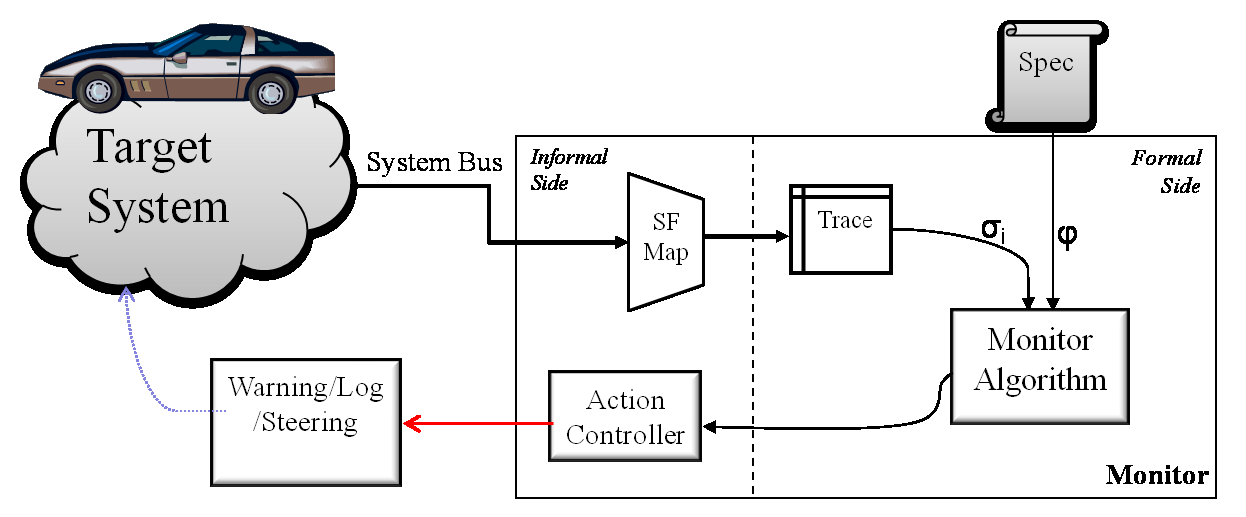
\includegraphics[width=4.5in]{img/mon_arch}
\caption{External monitor architecture outline \label{fig:architecture}}
\end{figure}

This architecture separates the system-independent formal aspects of the monitor from the system-dependent components including the semi-formal interface and system configurations. 
%By utilizing a semi-formal interface, we can separate the formal aspects of the monitor, which are completely independent from the target system, from the more practical pieces: the monitor interfaces and their configurations, which are system dependent. 
This allows us to utilize a core formal monitoring algorithm and framework with any system where an interface map can be used to create a state snapshot. 
Separating the system dependent and system-independent aspects of the monitor also lets the high level system requirements be somewhat abstracted away from the implementation. This means that changes to the target system may only require changes to the interface configuration and not the high level system specification. This is a similar situation to the two-level specifications used in the MaC framework \cite{Kim2004}.

\subsection{Semi-formal Monitoring}
Using formal methods has some clear benefits such as removing ambiguity, enabling early defect identification and allowing automated checking of properties. Even so, industrial adoption of formal methods, especially in software and system engineering has been slow (with hardware design being an exception) due to well known challenges such as a lack of tools and difficulty integrating with real systems \cite{Knight1998}. 
%
With regards to formal specifications, one possible cause is that completely describing a real system in most formal languages can be difficult or imposible. This is a part of Knight et al's formal specification evaluation criteria \emph{coverage}, which notes that a formal specification must permit description of all of an application or be designed to operate with any other notations that will be required \cite{Knight1997a}. 
This is a key concept for any practical and general runtime verification framework for real-world systems. Different systems will have varying specification needs, and if these needs are not easily met history shows that system designers are likely to just use an informal specification instead, which restricts the use of formal verification techniques.

To ensure specification flexibility, we have implemented a semi-formal specification which combines a formal specification with a semi-formal \emph{system mapping} which translates the actual system values into the monitor's more abstract execution trace. 
This semi-formal interface allows considerable leeway in designing the translation between the system and monitor's model. This leeway is both powerful and potentially dangerous. 
By allowing certain transformations in the interface, we are able to remove complexity from the monitor itself while ensuring that we can monitor a diverse set of needs.
This approach needs to be used carefully because it shifts part of the specification away from being formally defined, creating more opportunity for design mistakes and eroding some of the benefits that lead us to formal runtime verification in the first place.

%@PHIL need figure that summarizes this section
The two part specification feeds into two parts of the monitor, as shown in Figure \ref{fig:arch:arch_config}. 
The high-level formal specification contains the formal logic formulas that are directly checked by the formal monitoring algorithm.
The lower-level semi-formal mapping is used to define the system to monitor interface which generates the formal trace propositions that are checked by the monitoring algorithm. From an framework perspective, the semi-formal interface has minimal design constraints. 
As long as the interface provides a system trace of the properties present in the formal specification, we do not restrict how this trace is created.
%The interface can do any complex computations as long as it provides a system trace of the properties present in the formal specification. 

\begin{figure}
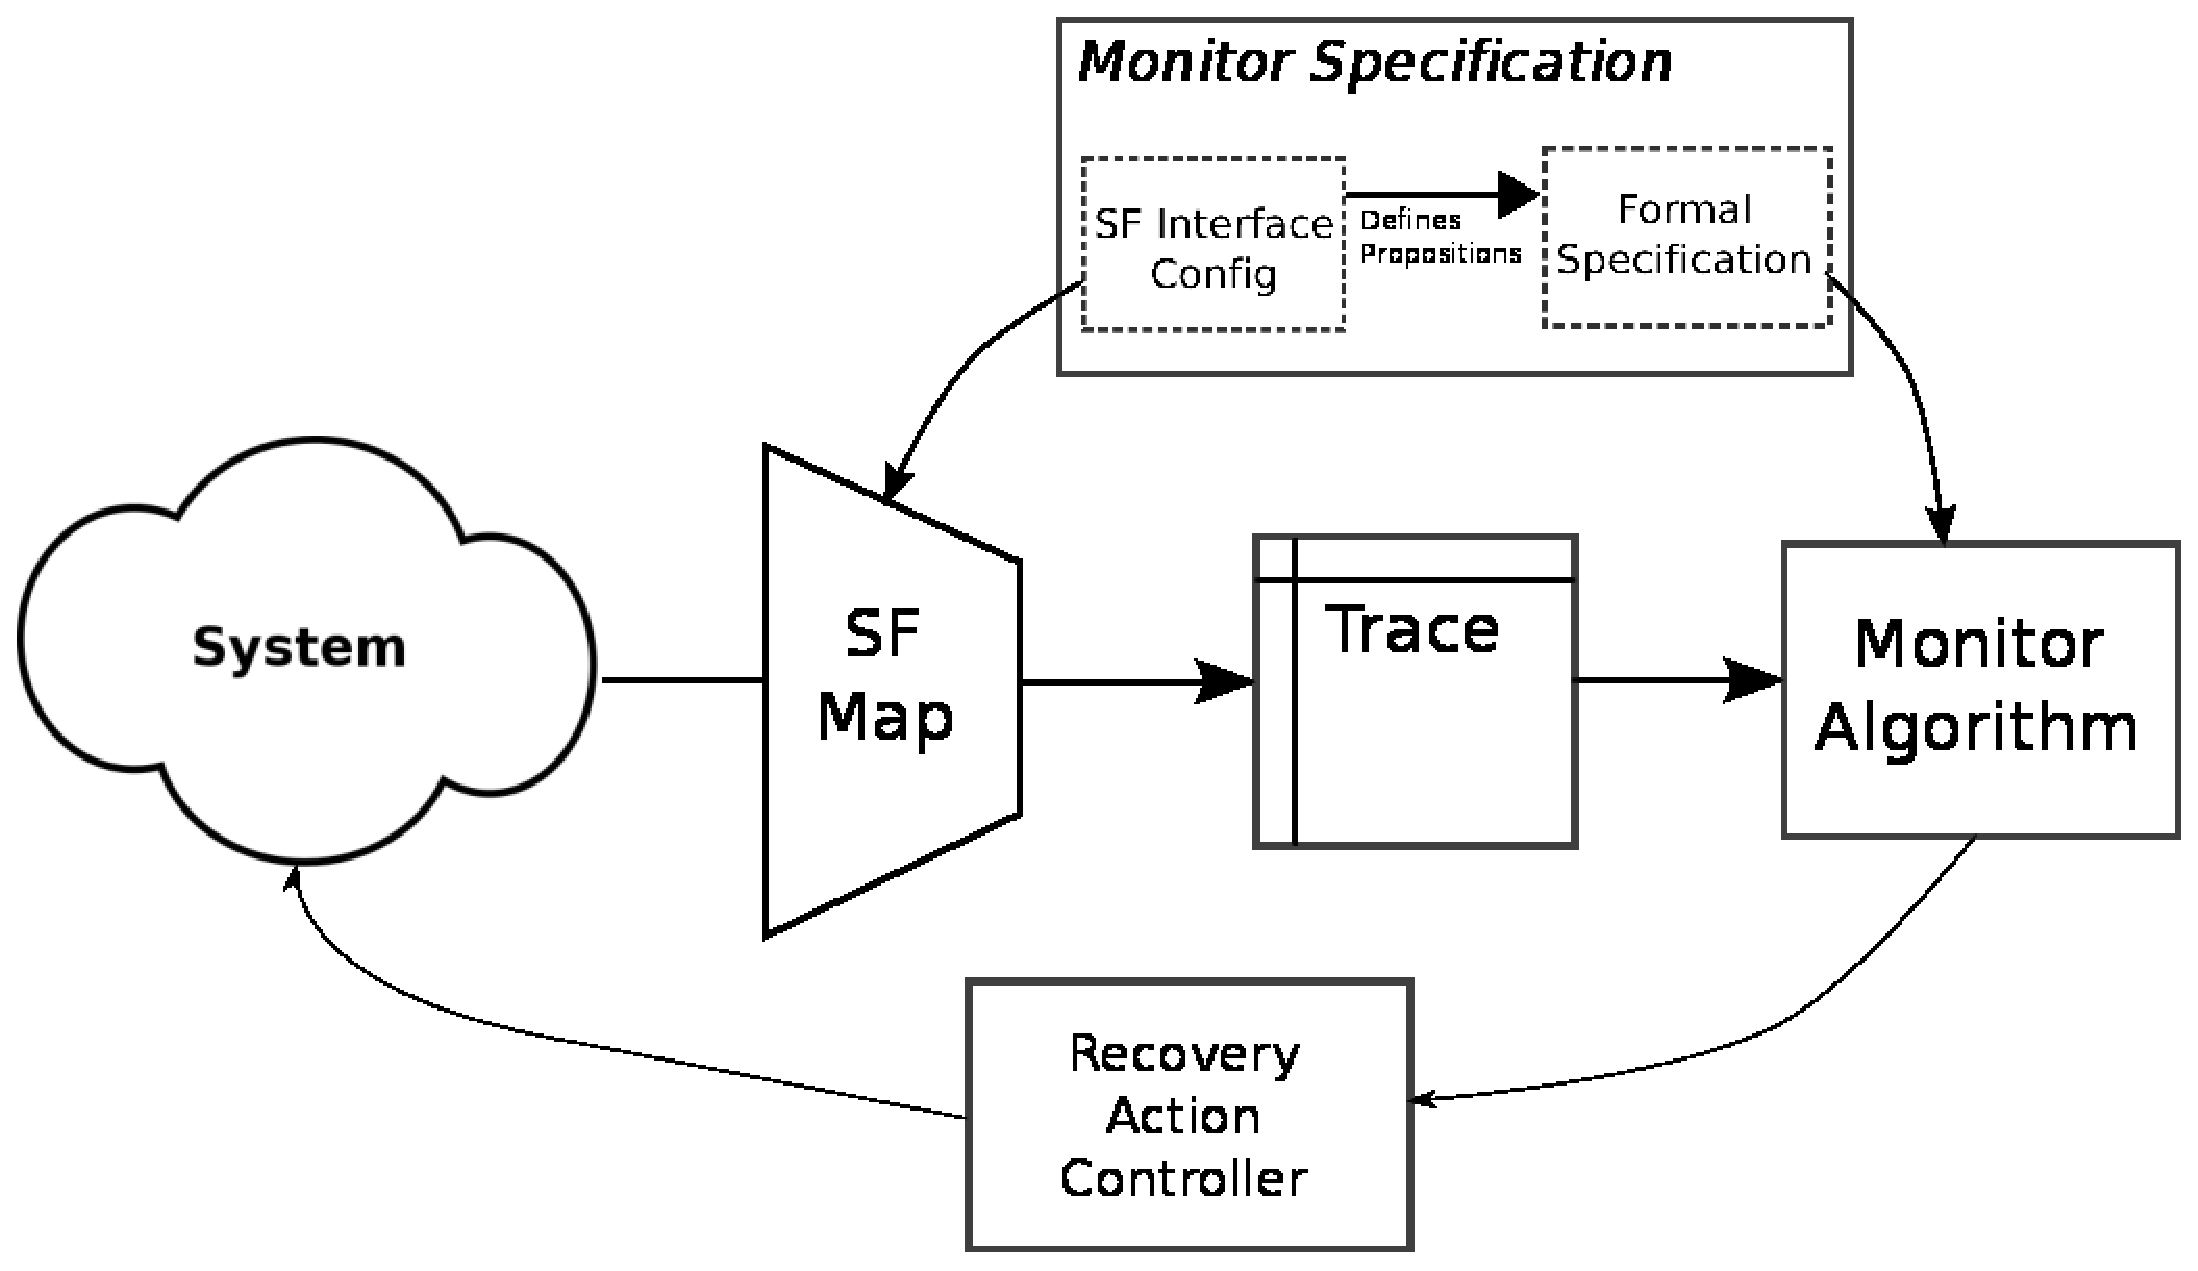
\includegraphics[width=4.5in]{img/arch_config}
\caption{Monitor architecture showing multi-part specification \label{fig:arch:arch_config}}
\end{figure}
Because the correctness of the monitor ultimately relies on the correctness of the interface transformations, limiting the interface to a simple, verifiable set of transformations is key to providing guarantees about the monitor's output.

The interface has two primary purposes: 

\begin{enumerate}
	\item To convert actual system values (e.g., network message data) into a propositional execution trace. 
	%\item To map these network messages onto specification propositions
	\item To provide additional semantic power to create useful propositions (e.g., state machines).
\end{enumerate}

The interface translates observable system state into a trace of propositions which can be checked against a specification by our monitoring algorithm. 
%
The interface provides the ability to extract the relevant data out of network messages in a flexible, network agnostic way. It can be used to extract the desired portion of a message, change units or typecast as necessary and then store the created proposition value correctly for use with the monitor. This ensures that the monitor is not restricted to networks or message types that it already knows how to transform. Any necessary data transformations can also be done in the interface.
%
Besides simple transformations (e.g., storing boolean values into propositions, arithmatic comparisons, etc.), we can also do more complex compututations and conversions in the interface such as building state machines whose state can be used to fill propositions.
%Besides relatively obvious transformations (status booleans into propositions, arithmatic comparisons) we can also do some slightly more complex computing in the interface such as building state machines and providing their value as a proposition.

\subsection{Semi-Formal Interface Design}
The semi-formal interface is used provide the monitoring algorithm with the state trace.
There are no inherent limitations on the semi-formal interface besides that it must create a viable trace for the monitor.
%As long as it provides the monitoring algorithm a viable state, the monitor will work. 
There is, however, a practical limitation -- the more complex the interface becomes the less confidence we should have that it works correctly.
Given this, we'd like to restrict the interface as much as possible while still providing the necessary flexibility.
% so we 

From our experience with system requirements and monitoring, the important transformations that are common for these types of systems are simple arithmetic, boolean connectives, comparisons to recent values, and simple state machines. 
%
Because of this, we restrict our own semi-formal mapping syntax to a simplified subset of the C programming language. We allow all the basic algorithmic, bitwise, and comparison operators and statically allocated variables of primitive types (i.e., integers, floating point).
We do allow simple loops, for example over a static array holding a set of values, for calculating averages and other simple values.
We do not currently have a formal definition of the semi-formal syntax, instead we trust that users can decide how restricted they wish to and realistically can be.

%Knowing this we can define a restricted semi-formal syntax based on the semantics of the C programming language, shown in Figure \ref{fig:arch:sfm_syntax}.
%
Our monitor implementation's semi-formal mapping configuration is integrated into the monitor's code directly by a specification compiler. 
This is essentially an internal domain specific language (DSL) \cite{Barringer2012}. 
Using a DSL to specify the semi-formal mappings allows us to restrict the specification of the interface to keep verification (of the interface) reasonable while still providing the ease of use and power of a programming language. 
Other prototype monitors we designed have used more traditional interface DSLs where the specifications have been used to insert and generate the code used by the monitor for the interface. 
More discussion about using domain specific languages for the semi-formal interface is included in Section \ref{sec:discussion:dsl}.

%%%% sfm_syntax\ldots
%\begin{figure}
%var ::= int | bool | \ldots \\
%SFM ::= var | var+var | var*var | \ldots \\
%\caption{Restricted Semi-Formal interface syntax \label{fig:arch:sfm_syntax}}
%\end{figure}

% describe the syntax\ldots
The motivation behind the restricted interface syntax is to provide enough power to define the system propositions necessary to monitor any reasonable desired property while incentivizing the monitor designers to work within the formal specification as much as possible.
%
Given a desired set of system properties, it is easy to imagine the pathological case where the monitor is configured to check the proposition \texttt{SystemOK} and the interface is built to compute this value directly. While this technically would work, it is obviously an abuse of the interface and a bad (non?) use of the monitor framework. Doing this essentially creates a completely informal monitor inside the interface, wasting the proven correctness of the formal monitoring algorithm.

A more interesting case is when we have a system message which includes a value and a validity bit (signifying whether the message value is valid). 
We can imagine that most rules utilizing this value will want to check both some property of the value and whether it is valid at the same time (e.g., \texttt{valuePositive} and \texttt{valueValid}). 
This could be done on the formal side in the logic by using $\texttt{valuePositive} \wedge \texttt{valueValid}$ or by combining them in interface into one proposition $\texttt{valuePositiveValid}$ which is calculated from both incoming values. 

In this case it is less clear which method is superior, but we can suggest a few heuristics to help decide. Perhaps the most straightforward way to choose is to attempt to mirror the design documentation and requirements in the monitor specification. 
If the system requirements mention the validity either explicitly (as a message value) or implicitly (by mentioning a ``valid positive value'') then the monitor specification should also directly mention validity and use the validity message value directly. 
If the requirements do not mention validity, then we can treat validity as an implementation detail and hide it away in the interface's proposition transformation. 
This follows the idea that the high-level requirements are abstracted away from the implementation. So if the validity bit is an artifact of the implementation then it is intuitive to deal with it in the interface, but if the validity bit is a part of the higher level system design then it should also be a part of the monitor specification.

Other factors can also affect the decision, such as monitoring complexity (moving transformations to the interface can reduce the amount of work the monitoring algorithm has to do) or the desire to maximize the amount of monitoring that is formally performed. 
These decisions should be kept consistent across specification rules to avoid confusion or misunderstanding.

%@PHIL -- need a paragraph about best way to use layered approach
In an ideal situation, the formal specification would contain all the relevant safety specification parts, leaving only the actual translation of system values to the semi-formal interface. 
More complex translations than simple threshold comparisons or copying booleans may require some semi-formal transformation if the desired properties cannot be expressed in propositional logic. 
%The bare minimum transformations needed to build the necessary propositions should be used, keeping as much of the verification in the formal side as possible. 
Moving parts of the transformation to the interface side is useful when necessary, but as the interface configuration complexity increases it becomes more important to validate and verify the interface itself.

%%@TODO mapping problems -- sampling periods and discrete value jumps
%% 	not sure if they go here or elsewhere, leaving note for now


%% andre notes
% system level spec is overapproximation? but! avoids the complexity of software
% what do people want from a semiformal map
%% can we say anything mathematically -- if you don't use something safe you don't have any guarantees


%%%%%%%%%%%%%%%%%%%%%%%%%%%%%%
%%% going to be way too long to copy without reformatting, but let's see
%%%%%%%%%%%%%%%%%%%%%%%%%%%%%%%%%%%%%%%

\section{Monitoring Algorithm}
The monitoring algorithm is an aggressive, iterative algorithm based on formula reduction (essentially formula-rewriting) and a stored history structure to check whether a given formula satisfies or violates the target trace. 
It is aggressive in that the algorithm attempts to check future-time temporal formulas as soon as possible rather than wait until an answer is guaranteed to be available (by combining short-circuiting and immediate checking of temporal subformulas).
This is in contrast to many existing runtime monitoring algorithms which either are restricted to past time logics (in which there is no waiting) or only check properties after their available delay. % some aggressive future time algorithms exist but almost always dynamic programming so can't do windowed bounds
The algorithm is iterative in that the history structure must be updated at each timestep in the trace in order. 

\subsection{Specification Logic}
The specification logic is built upon a set of atomic propositions which represent system properties (e.g., a proposition $speedLT40mph$ stating that the vehicle speed is less than 40mph). These propositions are created from the observable system state by the semi-formal interface.
Let $AP$ be the set of atomic propositions. 
%These propositions are the actual system state propositions which we will monitor (e.g., $speedLT60mph$). 
A \emph{state} $s: AP \rightarrow \{\top,\bot\}$ is a mapping from $AP$ to the set of truth values. A \emph{trace} $\sigma = s_0s_1s_2\ldots{}s_n$ is a finite sequence of states. We use $\sigma_i$ to denote the state $s_i$ at position $i$ in $\sigma$.
%
A time series $\tau = t_0t_1t_2\ldots{}t_n$ is a finite series of timestamps $t\in\mathbb{T}$. The pair $\sigma, \tau$ together represent a timed trace where each timestamp $\tau_i$ is the time associated with the occurance of state $s_i$.
%A timed trace $\rho = (\sigma, \tau)$ is a tuple containing a trace and a time series where each $\tau_i$ is the timestamp for which the new state $\sigma_i$ was obtained. 
%
%We use $\sigma_{\tau}(p)$ to denote the truth value of $p$ at time $\tau$, that is $\forall \tau \in [t_0, t_n]$ where $\tau \in [t_i, t_{i+1})$: $s_{\tau}(p) \equiv s_i(p)$ (for $n = |\sigma|$ and $t_{n +1}$ treated as $\infty$).

\subsection{Specifications}
\label{sec:formal:spec}
A \emph{specification} is a set of system invariants written in our bounded MTL variant BMTL which is a past- and future-time MTL with only finite intervals.  
We refer to the invariants as the specification \emph{rules} or \emph{policies}. The specification rules are checked at every monitored step, so each rule has an implicit unbounded \emph{always} over it (similar to safety rules in \cite{Basin2008}). The syntax of BMTL is shown below:
%there is an implied unbounded \emph{always} operator over all rules (which is what makes them invariants). 

%% syntax goes here\ldots
%Our language syntax is
$$\psi ::=  p \, | \,  \neg \psi \, | \,  \psi_1 \vee \psi_2 \, | \,  \psi_1 \mathcal{U}_{[l,h]} \psi_2 \, | \, \psi_1 \mathcal{S}_{[l,h]} \psi_2$$

Policy formulas are denoted by $\psi$. Policy formulas can include two bounded temporal operators: the past-time operator \emph{since} ($\mathcal{S}$) and the future-time operator \emph{until} ($\mathcal{U}$). 
%The \emph{until} operator states that $\psi_1$ must be true until (but not including) the time step when $\psi_2$ is true within the time bounds $[l,h]$.
Both temporal operators include a time bound interval $[l,h]$ where $l,h \in \mathbb{T}$ and $0 \leq l \leq h$. 
These intervals bound the time in which the triggering subformula $\psi_2$ is evaluated. 
An \emph{until} formula $\alpha\, \mathcal{U}_{[l,h]}\, \beta$ states that $\alpha$ must be true from the current step $i$ until (but not including) the time step $k$ where $\tau_k \in [\tau_i+l,\tau_i+h]$ and $\beta$ is true. 
\emph{Since} formulas are similar but in the past: $\alpha\, \mathcal{S}_{[l,h]}\, \beta$ states that $\alpha$ must have been true since (but not including) timestep $k$ where  $\tau_k \in [\tau_i-h,\tau_i-l]$ and $\beta$ was true (where $i$ is the current time step).

%For example, the formula $\alpha\, \mathcal{U}_{[3,5]}\, \beta$ means that $\beta$ must occur at some point within 3 to 5 time units, and $\alpha$ must be true from the current time until that point. 
Specification policies are interpreted over a timed system trace $\sigma,\tau$. 
%and associated timestamp series $\tau$. 
%Each state $s_i$ in $\sigma$ has an associated timestamp $\tau_i$ in $\tau$. 
%which represents the time at which the state $s_i$ began. 
We write $\sigma, \tau, j \vDash \varphi$ to represent that the policy $\varphi$ is satisfied by the timed trace $(\sigma, \tau)$ at trace position $j$. We use a common definition of $\vDash$ defined inductively as follows:

%The semantics of our language are defined inductively as follows:

%%@TODO Probably need to do sig,tau,j \vDash so proofs are less confusing
\begin{align*}
% true
\sigma, \tau, j &\vDash \top & &\\
% prop
\sigma, \tau, j &\vDash p & \text{ if and only if } & \sigma_{j}(p) = \top \\
% or
\sigma, \tau, j &\vDash \neg \psi & \text{ if and only if } & \sigma, \tau, j, \nvDash \psi \\
% not
\sigma, \tau, j &\vDash \psi_1 \vee \psi_2 & \text{ if and only if } & \sigma, \tau, j \vDash \psi_1 \text{ or } \sigma, \tau, j \vDash \psi_2 \\
%% until
\sigma, \tau, j &\vDash \psi_1 \mathcal{U}_{[l,h]} \psi_2 & \text{ if and only if } 
	& \exists k: (l \leq \tau_k-\tau_j \leq h), \sigma, \tau, k \vDash \psi_2  \\
	& & & \text{ and } \forall k': (\tau_j \leq \tau_{k'} < \tau_k), \sigma, \tau, k' \vDash \psi_1 \\
%% since
\sigma,\tau, j &\vDash \psi_1 \mathcal{S}_{[l,h]} \psi_2 & \text{ if and only if } 
	& \exists k:  (l \leq \tau_j - \tau_k \leq h),  \sigma, \tau, k \vDash \psi_2 \\
	& & & \text{ and } \forall k': (\tau_k < \tau_{k'} \leq \tau_j), \sigma, \tau, k' \vDash \psi_1 \\
\end{align*}


%Note that we use the common definitions of \emph{until} and \emph{since} which do not require the propositions to overlap. For example, for $\alpha \mathcal{U}_{[0,3]} \beta$ at time $0$, if $\beta$ is true at time $2$, then $\alpha$ only needs to be true at times $0$ and $1$ (not also at $2$). The \emph{since} operator is similar ($\alpha$ does not need to be true at the time $\beta$ is).

We use the usual notational conveniences for the other common logic operators: \emph{eventually} ($\lozenge_{[l,h]} \psi \equiv \top\, \mathcal{U}_{[l,h]} \psi$), \emph{always} ($\square_{[l,h]} \psi \equiv \neg \lozenge_{[l,h]} \neg \psi$), \emph{past eventually} ($\blacklozenge_{[l,h]} \psi \equiv \top\, \mathcal{S}_{[l,h]} \psi$), \emph{past always} ($\blacksquare_{[l,h]} \equiv \neg \blacklozenge_{[l,h]} \neg \psi$) and the boolean connectives \emph{and} and \emph{implies} ($\wedge, \rightarrow$). 



\subsection{Definitions}
\paragraph{Residues}
A residue $r^j_{\phi} = \rpt{j}{\psi}{\phi}$ is a tagged pair where $j \in \mathbb{N}$ is a position in the trace and $\psi, \phi$ are well-formed formulas. The monitoring algorithm is built on these residual formulas which are used to represent the currently unreducable fragments of a given parent formula. 
The formula $\psi$ represents the known value of formula $\phi$ at time $j$. So $\psi$ is a shorter equivalent form (reduced formula) of $\phi$ at $j$. 
Residues are used to hold the history information of a formula at a specific time for checking temporal formula.
The $\mathbf{reduce}$ function performs formula rewriting by reducing a given residue based on the current state and history information. 


\paragraph{History Structures}
A history structure $S_{\phi}^i = \{ r_{\phi}^0, r_{\phi}^1, \ldots r_{\phi}^i \}$ is a list of residues which is used to store the history of a formula. This history is used as the state history log to check temporal formula. 

We let $\mathbb{S}^i_{\phi}$ represent the set of history structures for all temporal subformula of $\phi$, i.e., $\mathbb{S}^i_{\phi} = \bigcup_{\psi \in \mathbf{tempSub}(\phi)} S^i_{\psi}$.

\paragraph{Formula Delays}
There are two important delay functions that are used for this monitor. The first is the wait delay $\Delta^{\omega}(\phi)$, which defines an upper bound on the maximum time the monitor needs to wait before $\phi$ can be evaluated.
%
%@EDIT storage requirements of what?
The second delay function $\Delta^{S}(\phi)$ defines the storage requirements for the history structure $S_\phi$.


%%% Delta^w
\begin{align*}
\Delta^{\omega}(\phi) = \left\lbrace
\begin{aligned}
0 & \quad \text{ iff } \psi \equiv \top \\
0 & \quad \text{ iff } \psi \equiv \bot \\
0 & \quad \text{ iff } \psi \equiv p \\
\Delta^w(\psi) & \quad \text{ iff } \phi \equiv \neg \psi \\
%max(\Delta(\alpha),\Delta(\beta)) & \quad \text{ iff } \phi \equiv \alpha \wedge \beta \\
max(\Delta^w(\alpha),\Delta^w(\beta)) & \quad \text{ iff } \phi \equiv \alpha \vee \beta \\
%max(\Delta(\alpha),\Delta(\beta)) & \quad \text{ iff } \phi \equiv \alpha \rightarrow \beta \\
%H + \Delta(\psi) & \quad \text{ iff } \phi \equiv \square_{l,H} \psi \\
%h + \Delta(\psi) & \quad \text{ iff } \phi \equiv \lozenge_{l,h} \psi \\
h + max(\Delta^w(\alpha),\Delta^w(\beta)) & \quad \text{ iff } \phi \equiv \alpha\, \mathcal{U}_{[l,h]}\, \beta \\
%\Delta(\psi) & \quad \text{ iff } \phi \equiv \blacksquare_{l,H} \psi \\
%\Delta(\psi) & \quad \text{ iff } \phi \equiv \blacklozenge_{l,h} \psi \\
max(\Delta^w(\alpha),\Delta^w(\beta)) & \quad \text{ iff } \phi \equiv \alpha\, \mathcal{S}_{[l,h]}\, \beta \\
\end{aligned} \right. 
\end{align*}


%%% Delta
\begin{align*}
\Delta^{S}(\phi) = \left\lbrace
\begin{aligned}
0 & \quad \text{ iff } \psi \equiv \top \\
0 & \quad \text{ iff } \psi \equiv \bot \\
0 & \quad \text{ iff } \psi \equiv p \\
\Delta(\psi) & \quad \text{ iff } \phi \equiv \neg \psi \\
%max(\Delta(\alpha),\Delta(\beta)) & \quad \text{ iff } \phi \equiv \alpha \wedge \beta \\
max(\Delta(\alpha),\Delta(\beta)) & \quad \text{ iff } \phi \equiv \alpha \vee \beta \\
%max(\Delta(\alpha),\Delta(\beta)) & \quad \text{ iff } \phi \equiv \alpha \rightarrow \beta \\
%H + \Delta(\psi) & \quad \text{ iff } \phi \equiv \square_{l,H} \psi \\
%h + \Delta(\psi) & \quad \text{ iff } \phi \equiv \lozenge_{l,h} \psi \\
h + max(\Delta(\alpha),\Delta(\beta)) & \quad \text{ iff } \phi \equiv \alpha\, \mathcal{U}_{[l,h]}\, \beta \\
%\Delta(\psi) & \quad \text{ iff } \phi \equiv \blacksquare_{l,H} \psi \\
%\Delta(\psi) & \quad \text{ iff } \phi \equiv \blacklozenge_{l,h} \psi \\
max(\Delta(\alpha),\Delta(\beta)) & \quad \text{ iff } \phi \equiv \alpha\, \mathcal{S}_{[l,h]}\, \beta \\
\end{aligned} \right. 
\end{align*}


\paragraph{Simplify}
The $\mathbf{simplify()}$ function is used to rewrite a given formula in a syntactically reduced form. For the restricted logic, simplify only rewrites two types of formulas. It removes \emph{not}s from formulas when the truth value is known and reduces \emph{or} formulas based on any known truth values. 

%@EDIT- fix layout -- do T if phi = (T \vee \phi) or (\phi \vee T)
%%%%%%%%%%%%%%%%%%%%%%%%%%%%%%%%%%%%%%
%%%% simplify
\begin{align*}
\mathbf{simplify}(\phi) = \left\{
\begin{aligned}
&\top &\text{ if } \phi \equiv \neg \bot \\
&\bot &\text{ if } \phi \equiv \neg \top \\
&\top &\text {if } \phi \equiv \psi_1 \vee \psi_2 \\
& &\text{ and } \\ & & \psi_1 \equiv \top \text{ or } \psi_2 \equiv \top \\
&\psi_1 &\text{ if } \phi \equiv \psi_1 \vee \bot \\
&\psi_2 &\text{ if } \phi \equiv \bot \vee \psi_2 \\
&\phi &\text{ otherwise}
\end{aligned} \right. \\
\end{align*}

\paragraph{Subformulas of Temporal Formulas}
The only trace history that needs to be saved for later use when monitoring this logic is the history of the direct child formulas of temporal formula. That is, for $\alpha\, \mathcal{U}_{[l,h]}\, \beta$ we need to save the history of $\alpha$ and $\beta$ (and if either of those are also a temporal formula then we need their history as well). The function $\mathbf{tempSub}(\psi)$ returns a list of all the subformula of $\psi$ that need their history to be saved.

%%%%%%%%%%%%%%%%%%%%%%%%%%%%%%%%%%
%%% temp_sub
\begin{align*}
\mathbf{tempSub}(\psi) = \left\lbrace
\begin{aligned}
\emptyset & \quad \text{ if } \psi \equiv p \\
\{\psi_1\} \cup \{\psi_2\} \cup \mathbf{tempSub}(\psi_1) \\
\cup \mathbf{tempSub}(\psi_2) & \quad \text{ if } \psi \equiv \psi_1 \mathcal{U}_{[l,h]} \psi_2 \text{ or } \psi \equiv \psi_1 \mathcal{S}_{[l,h]} \psi_2 \\
\mathbf{tempSub}(\psi_1) \cup \mathbf{tempSub}(\psi_2) & \quad \text{ if } \psi \equiv \psi_1 \vee \psi_2 \\
\mathbf{tempSub}(\psi_1) & \quad \text{ if } \psi \equiv \neg \psi_1
\end{aligned} \right.
\end{align*}


%%% length
\paragraph{Formula Length}
The length $|\phi|$ of a formula $\phi$ is defined as the number of nodes in a formula: 
\begin{align*}
|\phi| = \left\lbrace
\begin{aligned}
1 & \quad \text{if } \phi \equiv p \\
1 + |\phi'| & \quad \text{if } \phi \equiv \neg \phi' \\
1 + |\alpha| + |\beta| & \quad \text{if } \phi \equiv \alpha \vee \beta \\
1 + |\alpha| + |\beta| & \quad \text{if } \phi \equiv \alpha\, \mathcal{U}_{[l,h]}\, \beta \\
1 + |\alpha| + |\beta| & \quad \text{if } \phi \equiv \alpha\, \mathcal{S}_{[l,h]}\, \beta \\
\end{aligned} \right.
\end{align*}



\paragraph{Incrementing History Structures}
History structures are used to hold the history state of a given formula during monitoring.
When a new state is encountered, existing history structures need to be updated for this new state. This requires both reducing all the structures residues with the new state (to update them based on the new current state) as well as adding a residue for the current encountered state. The $\mathbf{incrS}(\dots)$ procedure performs this update, reducing all of a structure's residues as well as adding a reduced residue for the current state.

%% incrS
\begin{align*}
\mathbf{incrS}(S^{i-1}_\psi, \mathbb{S}^i_{\psi}, \sigma, \tau, i) = %\left\lbrace
%\begin{aligned}
\left(\bigcup\limits_{r \in S^{i-1}_{\psi}} \mathbf{reduce}(\sigma, \tau, \mathbb{S}^i_{\psi}, r)\right) \cup \mathbf{reduce}(\sigma, \tau, \mathbb{S}^i_{\psi}, \rp{i}{\psi})
%\end{aligned} \right.
\end{align*}


\paragraph{Monitor Algorithm}
The high level algorithm is shown in Figure \ref{fig:ag_algorithm}. First, the history structure $\mathbb{S}_{\varphi}$ is built by identifying the required history structures needed to check the policy $\varphi$ with $\mathbf{tempSub(\varphi)}$. 
The history of these subformula and the current state at any given step are the only history required by the algorithm. Once the structure $\mathbb{S}_{\varphi}$ is built, the monitoring loop begins. 
In each step, first all the history structures are updated with the current step of the trace. This is done in increasing formula size since larger formula can depend on the history of smaller formula which may be their subformula.
Each structure is updated using $\mathbf{incrS}(S^{i-1}_\phi,\mathbb{S}^i_\phi,\sigma,\tau,i)$ which reduces all residues in the structure and adds a reduced residue for the current trace step. 
Then, the same procedure is performed for the top level policy that is being monitored -- the policy's structure is updated with $\mathbf{incrS}(S^{i-1}_\phi,\mathbb{S}^i_\phi,\sigma,\tau,i)$.
Once updated, this structure is checked for policy violations (any false residues) before the algorithm continues to the next trace step.
%The last structure here is the structure for the top-level policy being monitored, so this structure is then checked for policy violations before the monitor algorithm continues to the next trace step.

% the top level formula is only distinctive because we treat it that way to help intuition
% we could instead define tempSub to also return psi
It is important to note that due to the recursive nature of the monitor algorithm, the top-level policy is treated exactly as any temporal subformula would be (which follows from the implicit \emph{always} on all policies) except that violations of the top level policy are reported. We separate incrementing the subformulas from the specification policies in the algorithm description for clarity only.

\begin{figure}
\begin{algorithmic}[1]
%\STATE Recognize formulas for which we build structures
\STATE For all recognized formulas $\psi \in \mathbf{tempSub}(\varphi)$: $S^{-1}_{\psi} \leftarrow \emptyset$
\STATE $i \leftarrow 0$
\LOOP
\STATE Extend $\sigma$ and $\tau$ with next event $(\sigma_i,\tau_i)$
%\STATE Obtain $(\sigma_i,\tau_i)$ from trace
\FOR{every $\psi \in \mathbf{tempSub}(\varphi)$ in increasing size}
	\STATE $S^i_{\psi} \leftarrow \mathbf{incrS(} S^{i-1}_{\psi}, \mathbb{S}^i_{\psi}, \sigma, \tau, i)$
	%\STATE $S^i_{\psi} \leftarrow \bigcup\limits_{r \in S^{i-1}_{\psi}} \mathbf{reduce}(\sigma_i, \tau_i, \mathbb{S}^i_{\psi}, r) \cup \mathbf{reduce}(\sigma_i, \tau_i, \mathbb{S}^i_{\psi}, \rp{i}{\psi})$
\ENDFOR
\STATE $S^i_{\varphi} \leftarrow \mathbf{incrS(} S^{i-1}_{\varphi}, \mathbb{S}^i_{\varphi}, \sigma, \tau, i)$
\FOR{all $\rp{j}{\bot} \in S^i_{\varphi}$}
\STATE \texttt{Report violation on $\sigma$ at position $j$}
\ENDFOR
\STATE $i \leftarrow i + 1$
\ENDLOOP
\end{algorithmic}
\caption{Aggressive Monitoring Algorithm}\label{fig:ag_algorithm}
\end{figure}

%@EDIT explain in text what parameters of reduce are
%% could be a subsubsection? then they all should be though


\paragraph{Reduce}
The $\mathbf{reduce}$ function is the backbone of the monitor algorithm. It takes a residue and the current trace state and returns the residue in a reduced form.

The $\mathbf{reduce}$ function takes the following parameters: the current state $\sigma_i$, the timestamp sequence $\tau$, the current step $i$, the set of history structures $\mathbb{S}^i_{\phi}$, and a residue $\rpt{j}{\psi}{\phi}$. $\mathbf{Reduce}$ returns a reduced residue $\rpt{j}{\psi'}{\phi}$. Note that for $\phi = \mathbf{reduce}(\alpha \mathcal{U}_{[l,h]} \beta)$ (and also \emph{since}) we know that $\mathbb{S}^i_\phi$ at least contains $S^i_\alpha$ and $S^i_\beta$ (and possibly other structures if there are temporal subformulaof $\alpha$ or $\beta$).

Most $\mathbf{reduce}$ operations are straightforward and common formula-rewriting reductions for MTL. The $\mathbf{reduce}$ operations for \emph{Until} and \emph{Since} are more complex since they utilize our history structures. We show the definition for \emph{Until} here, \emph{Since} is similar except looking backwards (time bounds and min/max flipped). See Appendix \ref{app:reduce} for the full $\mathbf{reduce}$ definition.

%%% TAU UNTIL
\begin{align*}
\mathbf{reduce}(\sigma_i,\tau, i,\mathbb{S}^i_{\alpha\, \mathcal{U}_{[l,h]}\, \beta} ,\rp{j}{\alpha\, \mathcal{U}_{[l,h]}\, \beta}) = \left\{
\begin{aligned}
&\text{let } a_a \leftarrow min(\{k | \tau_j \leq \tau_k \leq \tau_j+h  \wedge \rp{k}{\bot} \in S^i_\alpha \},i) \\ 
% a_u
%& a_u \leftarrow max({k| \tau_j \leq \tau_k \leq \tau_j+h \wedge \rp{k}{\alpha'} \in S^i_\alpha \wedge \alpha' \not\equiv \top},i) \\
& a_u \leftarrow max(\{k| \tau_k \in [\tau_j,\tau_j+h] \\
& \quad \quad \quad \wedge \forall k' \in [j,k-1].(\rp{k'}{\alpha'} \in S^i_\alpha \wedge \alpha' \equiv \top\},i) \\
% b_a
& b_a \leftarrow min(\{k | \tau_j+l \leq \tau_k \leq \tau_j+h \wedge \rp{k}{\beta'} \in S^i_\beta \wedge \beta' \neq \bot\}) \\ 
% b_t
&b_t \leftarrow min(\{k | \tau_j+l \leq \tau_k \leq \tau_j+h \wedge \rp{k}{\top} \in S^i_{\beta} \}) \\
% b_n
&b_n \leftarrow \top \text{ if } (\tau_i - \tau_j \geq \Delta^w(\psi)) \\
& \quad \quad \quad \wedge \forall k.(\tau_j+l \leq \tau_k \leq \tau_j+h). \rp{k}{\bot} \in S^i_{\beta} \\
&\text{if } b_t \neq \emptyset \wedge a_u \geq b_t \\
& \quad\mathbf{return} \rp{j}{\top} \\
&\text{else if } (b_a \neq \emptyset \wedge a_a < b_a) \text{ or } b_n = \top\\ & \quad\mathbf{return} \rp{j}{\bot} \\
&\text{else} \\
& \quad\mathbf{return} \rp{j}{\alpha\, \mathcal{U}_{[l,h]}\, \beta}
\end{aligned} \right. \\
\end{align*}

For residues whose formula is an \emph{until} formula $\alpha \mathcal{U}_{[l,h]} \beta$, the history structures $S^i_\alpha$ and $S^i_\beta$ are used to reduce the formula. 
If the formula can be evaluated conclusively then the truth value is returned, otherwise the residue is returned unchanged. 
We utilize five marker variables to evaluate the formula over the current trace: 
\begin{itemize}
\item $a_a$ is the earliest in-bounds ($[\tau_j,\tau_j+h]$) step at which $\alpha$ is false. This represents the latest time step at which $\beta$ can be true for $\alpha \mathcal{U}_{[l,h]} \beta$ to be true. 
\item $a_u$ is the latest in-bounds ($[\tau_j,\tau_j+h]$) step at which $\alpha$ has been true since the residue time step.  This represents the latest time step that the \emph{until} formula would be conclusively true if $\beta$ was true at that step. 
\item $b_a$ is the earliest in-bounds ($[\tau_j+l,\tau_j+h]$) step at which $\beta$ is not conclusively false. This is used to check whether the formula is still satisfiable or not.
\item $b_t$ is the earliest in-bounds ($[\tau_j+l,\tau_j+h]$) step at which $\beta$ is conclusively true.
\item $b_n$ is true if the current step is later than the wait delay $\Delta^w(\psi)$ of the residue and all residues in bounds are false (that is, $\beta$ is conclusively false at all steps in bounds).
\end{itemize}

Using these marker variables, we can evaluate the semantics of \emph{until}. If $a_u \geq b_t$ (and $b_t$ exists) then we know that $\alpha$ is true from the residue step $j$ until the step $b_t$ where $\beta$ is true, which satisfies the semantics of \emph{until} (so we return $\top$).
%
Otherwise, if $a_a < b_a$ then $\alpha$ is not true until the first possible step that $\beta$ could be true (since $b_a$ is the earliest non-false step). $\alpha \mathcal{U}_{[l,h]} \beta$ cannot be true in this case, so we return $\bot$. Similarly, if $b_n$ is true, then there is no $\beta$ in bounds and the formula is false.
%
If none of these cases exist then the trace is inconclusive, so the residue is returned unchanged.

%%%%%%%%%%%%%%%%%%%%%%%%%%%%
%%%%%%%%%%%%%%%%%%%%%%%%%%%%


\section{Monitor Implementation}
\subsection{Evaluation}
\label{sec:eval:embedded}
To evaluate the embedded monitor we need to check an actual CAN bus.  Since we did not have access to a real system with CAN and a data dictionary to monitor, we instead performed real-time replay of timestamped CAN logs captured during testing of a real system onto a bench CAN bus which the monitor was connected to, as shown in Figure \ref{fig:eval:replaySchem}. 

\begin{figure}
\centering
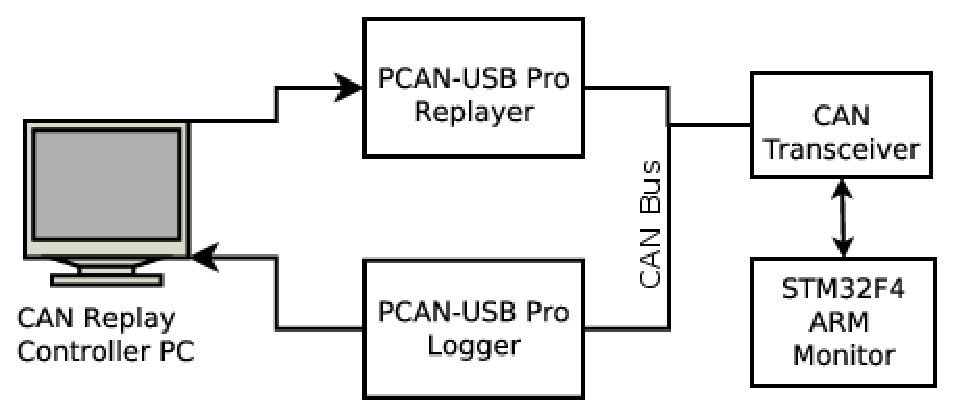
\includegraphics[width=4.5in]{img/replay_arch}
\caption{CAN replay setup \label{fig:eval:replaySchem}}
\end{figure}
%%% about SUT
The system under test that provided the logs is an autonomous heavy truck which is being designed for use in vehicle platoons. % cite/discuss AMAS/ASTAA?
The system has multiple internal buses, some CAN and some Ethernet, connecting different system components. The logs we monitor are from robustness testing of the interface controller, so we focus on its CAN bus which contains communication between the interface controller and the primary vehicle controller.
The logs contain both normal operation as well as some operation under injected robustness testing. During robustness testing, the testing framework can hijack targeted network messages on the bus to inject testing values. % could cite astaa here

A PC was connected to a PCAN-USB Pro \cite{PCAN-USBPro} device which provides a USB interface to two CAN connections. One CAN channel was used as the log replayer, while the other was used as a bus logger for analysis purposes.
%%% replay
We performed log replay with a PC-based script which would take a test log and replay it on the CAN bus based on the log's timestamps. A separate script used the second CAN connection to log the CAN network traffic.
The replay timing is based on a busy-wait using the log timestamps. 
We compared the replayed log timings to the original test logs to ensure this replay was accurate. 
The percent error in message timestamps relative to the start of the message in our longest logs had an average of less than 0.01\% error. The absolute error was generally sub-millisecond, which is accurate enough for our 25ms monitor with its greater than 50ms minimum time step resolution.

%Figure \ref{fig:eval:replay_timing} compares the replayed log timings to the actual test logs.
%D%\begin{table}
%D%\centering
%D%\begin{tabular}{|l|l|l|}
%D%\hline Log \# & Average delta error & average message error \\
%D%\hline 1 & -0.0005\% & \\
%D%\hline 2 & -0.00499\% & \\
%D%\hline
%D%\end{tabular}
%D%\caption{CAN Log Replay Timing Error}
%D%\label{tab:eval:replay_timing}
%D%\end{table}


%%%%%%%%%
%% rule elicitation
\subsection{Rule Elicitation}
For this system we did have requirements documentation which could more directly lead to a monitoring specification. 
%Due to the test focus for the logs we have, we mainly created specifications checking the user interface feature. 
Since we wanted to monitor the interface bus, we identified requirements which we could monitor or partially monitor based on the state available on this bus.
The specifications we used on the embedded monitor are shown in Table \ref{tab:eval:nrecrules} and the propositions used in these rules are described in Table \ref{tab:eval:nrecprops}.

\begin{table}
%\begin{tabular}{|p{3in}|l|}
\begin{tabular}{|l|p{5in}|}
\hline \multirow{2}{*}{Rule \#} & Informal Rule \\ & BMTL \\
%\hline Informal Rule & BMTL \\
%\hline \multirow{2}{*}{0} & A feature heartbeat shall be received every 500ms \\
%& $\lozenge_{[0,100ms]} HeartBeat$ \\
\hline \multirow{2}{*}{0} & A feature heartbeat shall be received every 500ms \\
& $HeartbeatOn \rightarrow \lozenge_{[0,500ms]} HeartBeat$ \\
\hline \multirow{2}{*}{1} & The interface component heartbeat counter is correct \\
& $HeartbeatOn \rightarrow HeartbeatCounterOk$ \\
%% make sure to put both status and command in here (maybe split them)
%\hline \multirow{2}{*}{2} & The vehicle controller shall not command a transition from manual mode to autonomous mode as seen on the interface component \\ 
\hline \multirow{2}{*}{2} & The vehicle shall not transition from manual mode to autonomous mode \\
&  $\neg ((\blacksquare_{[1,1]} IntManualState) \wedge IntAutoStat)$\\
\hline \multirow{2}{*}{3} & The vehicle controller shall not command a transition from manual mode to autonomous mode \\
& $\neg ((\blacksquare_{[1,1]} VehManualModeCmd) \wedge VehAutoModeCmd)$\\
\hline \multirow{2}{*}{4} & The vehicle shall not transition from system off mode to autonomous mode \\ 
&  $\neg ((\blacksquare_{[1,1]} IntSDState) \wedge IntAutoStat)$\\
\hline \multirow{2}{*}{5} & The vehicle controller shall not command a transition from system off mode to autonomous mode \\
& $\neg ((\blacksquare_{[1,1]} VehSDModeCmd) \wedge VehAutoModeCmd)$\\
% warn was at 200ms
\hline
\end{tabular}
\caption{CAN replay monitoring specification \label{tab:eval:nrecrules}}
\end{table}

The rules were derived from the vehicle safety requirements documentation. 
Limited to the observable state on the interface bus, we used the user interface LEDs as proxies for the actual system state. 
This is an approximation we would feel is reasonable in most systems, and in this case there were also safety requirements which state that the output LEDs should be correct. This provides us more assurance that the approximation is reasonable.

% describe rules
% hb rules
Rule \#0 is a heartbeat detection which ensures that the interface component is still running (essentially a watchdog message). Rule \#1 is a second component of this check. The system's heartbeat message contains a single heartbeat status bit which we checked directly in Rule \#0, but the message also has a rolling counter field. 
We used the semi-formal interface to create a proposition that represents whether the counter is incrementing correctly (i.e., one value at a time). To block false-positive violations during initialization, we blocked these rules from being checked until after the first heartbeat message was received by creating a guard proposition $HeartbeatOn$ with the semi-formal interface. 
%Initialization of the system and monitor's model can be troublesome for monitoring, especially in testing when missing or unfinished components cause the system to take more time to get to a stable, monitorable state.
Initialization issues are discussed in more detail in Section \ref{sec:eval:mon_init}. 

% transition rules
We also watched the system state for illegal state transitions. Although the actual mode decisions and commands are on a different bus, we can still monitor the system state through the user interface LEDs which show the mode state. 
We created rules for two of the illegal transitions, from manual mode to autonomous driving and from system off to autonomous driving. We independently checked both the vehicle controller's LED command messages and the interface's LED status message for these transitions.

% prop mappings
The proposition mappings here were straightforward. The LED command and status messages were single bit fields and we checked the heartbeat's single bit status message. We checked the rolling heartbeat counter for  consistency (i.e., that it counted up and wrapped correctly) by comparing it against the previously seen value in the semi-formal interface. We also created the guard $HeartbeatOn$ which is false until the first heartbeat message is seen, and true from then on. 
% This was necessary to handle initialization issues
Using a guard proposition is our primary method to implement unbounded since/until type rules within our bounded logic. If we had unbounded operators we could use the formula $(\lozenge_{[0,500]} Heartbeat)\; \mathcal{S}\; (Heartbeat)$ instead of a mode-based guard proposition, but without unbounded operators using guard propositions to enable or disable a formula is a reasonable replacement.

\begin{table}
\centering
\caption{CAN replay propositions}
\label{tab:eval:nrecprops}
\begin{tabular}{lp{2in}l}
\textbf{Proposition Name} & \textbf{System Variables} & \textbf{Mapping} \\
\hline $HeartBeat$ & Feature Status Message Heartbeat field & Fresh direct boolean \\
$HeartbeatOn$ & Interface HB message & System Mode \\
$HeartbeatCounterOk$ & Interface HB message & Comparison with Past Value \\
$VehManualModeCmd$ & Vehicle command message & Direct Boolean \\
$VehAutoModeCmd$ & Vehicle command message & Direct Boolean \\
$VehicleSDModeCmd$ & Vehicle command message & Direct Boolean \\
$IntManualStat$ & Interface status message & Direct Boolean \\
$IntAutoStat$ & Interface status message & Direct Boolean \\
$IntSDStat$ & Interface status message & Direct Boolean \\
\end{tabular}
\end{table}


%% replay
\subsection{Monitoring results}
We monitored the CAN log replays on our test CAN network with the specification discussed above.
%
To capture violations for analysis we configured the monitor to send a CAN message denoting the violated policy when violations were detected. These violation messages were rate limited to one message per second to allow the violation message to have a high CAN priority without letting it take over the network. 

The monitor found heartbeat violations in the logs captured during robustness testing. 
% covering all three possible violation types. One was a false positive
Three different types of heartbeat violations were identified after inspecting the monitor results.
% missing hb message
The first is a late heartbeat message. In one of the robustness testing logs the heartbeat message was not sent on time, which is clearly a heartbeat violation. Figure \ref{fig:eval:hb_arrival:vals} shows the heartbeat counter values and the inter-arrival time of the heartbeat messages over time for this violation. We can see here that the heartbeat counter did in fact increment in a valid way, just too slowly. 
%Figure \ref{fig:eval:hb_arrival:time} shows the inter-arrival time of these same messages.

\begin{figure}
	%\begin{subfigure}
		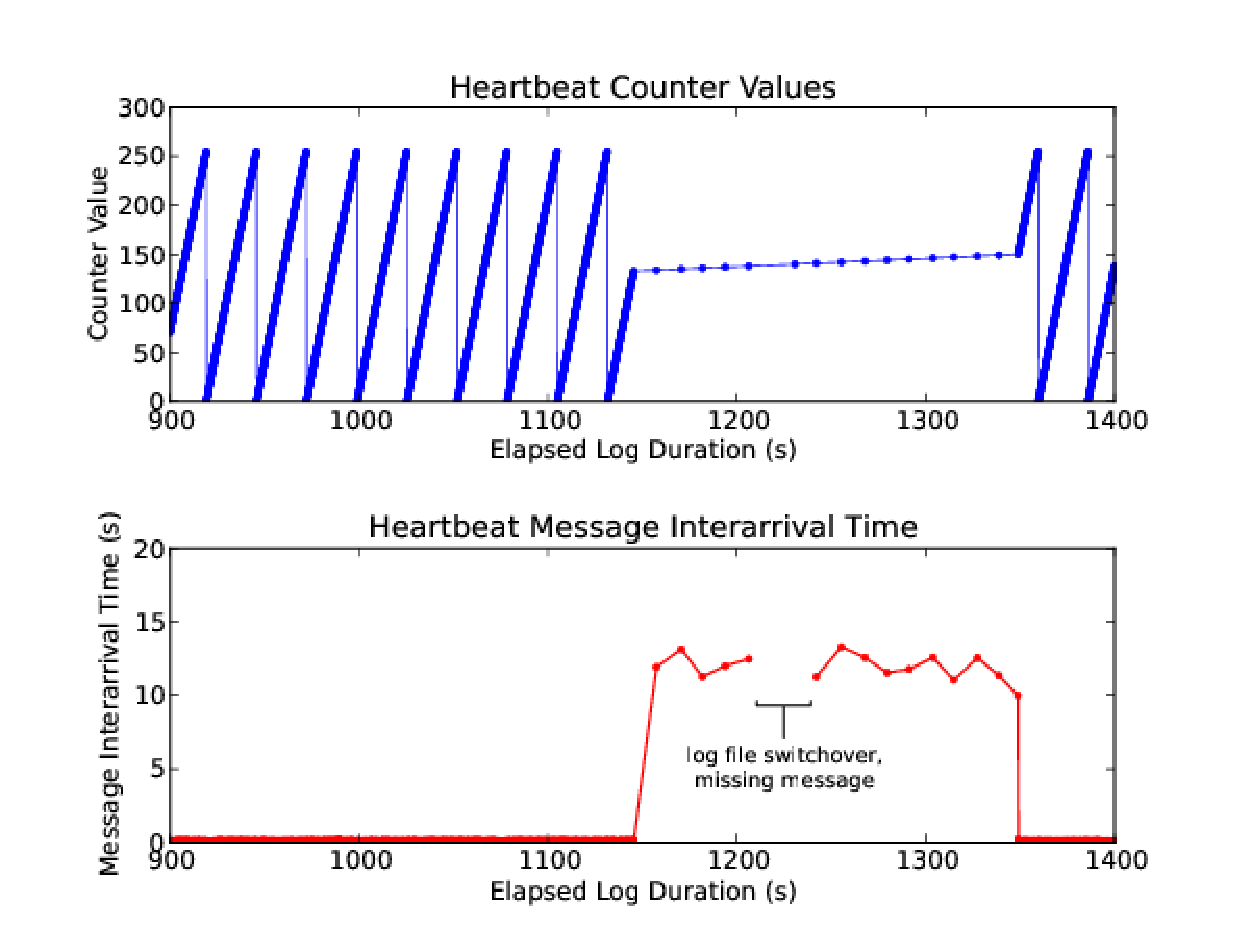
\includegraphics[width=4.5in]{img/hb1}
		%\includegraphics[width=6in]{img/fake_hb1}
		\caption{Heartbeat counter values over time}
		\label{fig:eval:hb_arrival:vals}
	%\end{subfigure}
\end{figure}
%\begin{figure}
%%	\begin{subfigure}
%%		%\includegraphics[width=6in]{img/hb}
%		\caption{Heartbeat counter message inter-arrival time}
%		\label{fig:eval:hb_arrival:time}
%	%\end{subfigure}
%\end{figure}
%%\caption{Bad Heartbeat Log}
%%\end{figure}

% bad status
The second violation is on-time heartbeat status message but the heartbeat status field is 0. 
We do not know from the available documentation whether a bad status in an on-time message with a good counter is valid or not. So without more information we cannot tell whether these violations are false positives or not. This is worthy of further investigation.

% bad counter
The last type of violation is a bad counter. 
We have defined a good counter as one which increments by one every message up to its maximum (255 in this case) before wrapping back to zero.
Every consecutive heartbeat status message must have an incremented heartbeat counter or a violation will be triggered. Figure \ref{fig:eval:hb_badcounter} shows the counter value history for one of the traces with a heartbeat violation caused by a bad counter value.
%
%@EDIT describe robustness testing, define these false positives like the talk?
Further inspection of this violation showed that the bad counter values were sent by the testing framework rather than the actual system. In this case, the network traffic the monitor is seeing is not real system state but actually it is messages being injected by the testing framework. This is not a real violation (since the violating state is not the actual system state), and so we consider this a false positive violation.
% this is a false positive

Different counter restrictions could also be used, such as allowing unchanging as well as incrementing values or requiring an increment to occur within a time threshold rather than every message. Once again, without documentation to point us towards the right restriction, all we can do is try a restriction and after seeing the monitoring results decide whether we believe our restriction is accurate or causes too many false positives. 
\begin{figure}
%includegraphics[width=5in]{img/hb_badcounter}
%\includegraphics[width=6in]{img/fake_hb2}
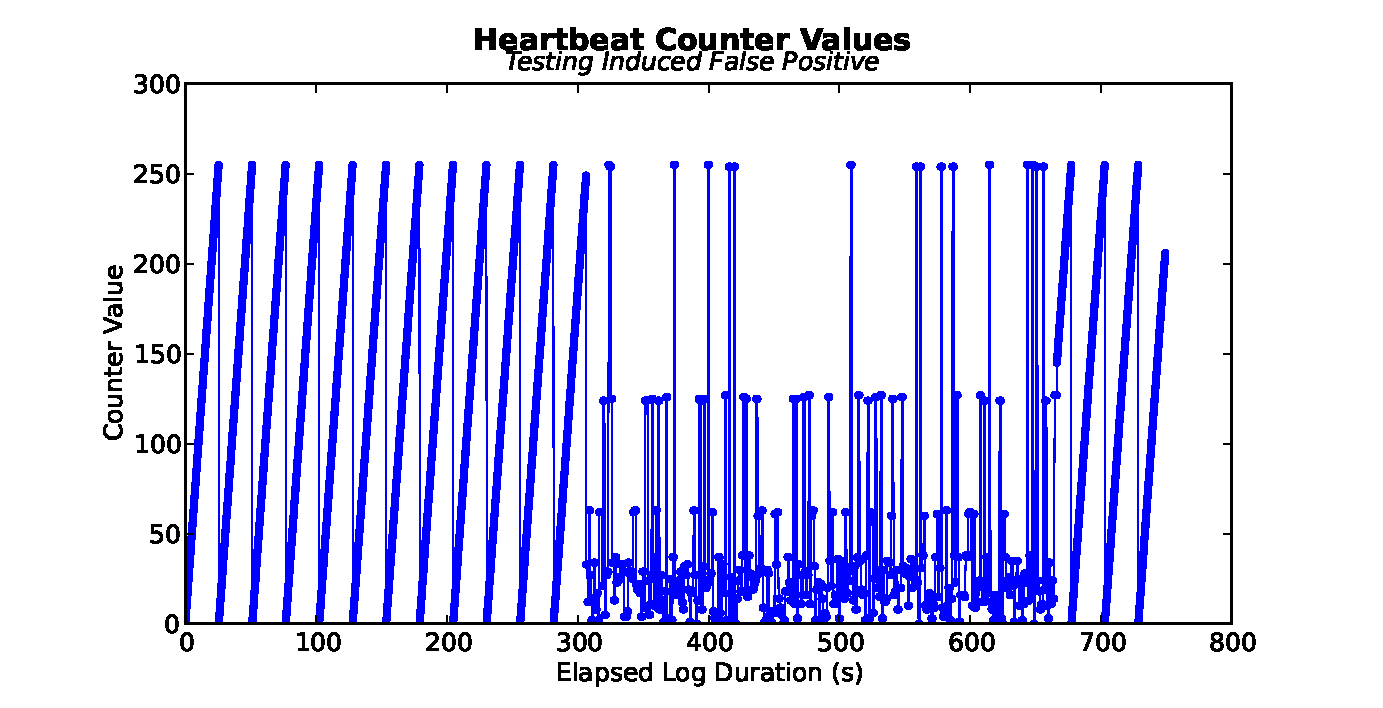
\includegraphics[width=4.5in]{img/hb2}
\caption{Bad heartbeat counter values \label{fig:eval:hb_badcounter}}
\end{figure}

%This was expected as these violations had been found with an offline monitoring tool previously.
There were also violations of the transition rules, but these, similar to the heartbeat counter violation, also turned out to be false positives triggered by message injections by the robustness testing harness. Since the monitor checks network state, if we perform testing that directly affects the values seen on the network (such as injection/interception of network messages) we may detect violations which are created by the testing framework rather than the system. 
%
This is a common issue when using monitors as a test oracle with some sort of fault or behavior injection -- the monitor needs to know which state is from the test and which is from the system. 
Information about the test configurations can be used to filter out these types of false positives which arise from test-controlled state.
%These types of false positives can be filtered out by using the test configurations to keep track of what system properties are being affected by the testing. 
This type of filtering can be automated if the test information can be input to the monitor, either directly on the network (e.g., adding a message value to injected messages) or through a side-channel (i.e., building a testing-aware monitor).

% detection time
Comparing the violation messages from the monitor with the actual network state we can see the monitor's detection speed. 
The deteection time for the monitor should approximately be the monitor's period plus the time to perform the monitoring and the time to send the detection message once the violation is detectable. 
This is approximately two monitoring periods (given that the time to send a high priority message is negligable). This bears out in the replay testing, where the violation messages come approximately 555ms after the last good heartbeat message, which is a 55ms response time and close to double the monitor's 25ms period.



\section{Conclusion}
The increase in use of third-party, black-box components in safety-critical systems increases the difficulty of verifying the safety and correctness of these systems. Runtime verification is a useful tool during testing and verification of these systems, but performing runtime monitoring of primarily black-box system's requires monitors which do not require instrumentation or source code access.

We have presented a semi-formal monitoring architecture for safety-critical systems made up of potentially black-box components. These monitors check externally observable system properties on a system's broadcast bus. A real-time embedded implementation of this monitor architecture for CAN has been evaluated against a bench CAN network using replayed logs from a research autonomous vehicle. The monitor identified specification violations in the logs in real-time.

%\def\IEEEbibitemsep{0pt plus .5pt}
\bibliographystyle{../llncs/splncs03}
% argument is your BibTeX string definitions and bibliography database(s)
\bibliography{../My_Collection}

\end{document}

